\documentclass[12pt]{article}
\usepackage{amsmath,amssymb,amsthm}
\usepackage{graphicx}
\usepackage{subcaption}
\usepackage{float}
\usepackage{hyperref}
\usepackage{color}
\usepackage{enumitem}
\usepackage{tabularx}
\usepackage[sorting=none]{biblatex}

% figure and bibliography source
\addbibresource{../prime-editing.bib}
% add figure path
\graphicspath{ {../figures/} }
% reduce margin
\usepackage[margin=1in]{geometry}
% increase title font size
\usepackage{titling}

\title{Project Proposal: Designing a Machine Learning Algorithm for Predicting the Outcomes of Prime Editing}

\begin{document}
\maketitle

\section{Background: The Theory or Application Areas}

Prime editing is a state of the art genetic editing technologies using the CRISPR-Cas9 platform. It is a versatile tool that can be used to add or delete sequences of varying lengths, as well as insert both transversion(G-C$\iff$C-G, A-T$\iff$T-A) and transition(A-T$\iff$G-C) mutation into designated positions of the genome. It does not introduce double strand break(DSB) like CRISPR system utilizing homology directed repair system(HDR), and thus would not be interfered by the cell's competing non-homologous end joining(NHEJ) repair pathway that leads to unwanted insertion/deletions(indels). It is also more versatile than base editing, which does not cause DSB but can only introduce point mutations\cite{liuPrimeEditingPrecise2023}.

\begin{figure}[ht]
    \centering
    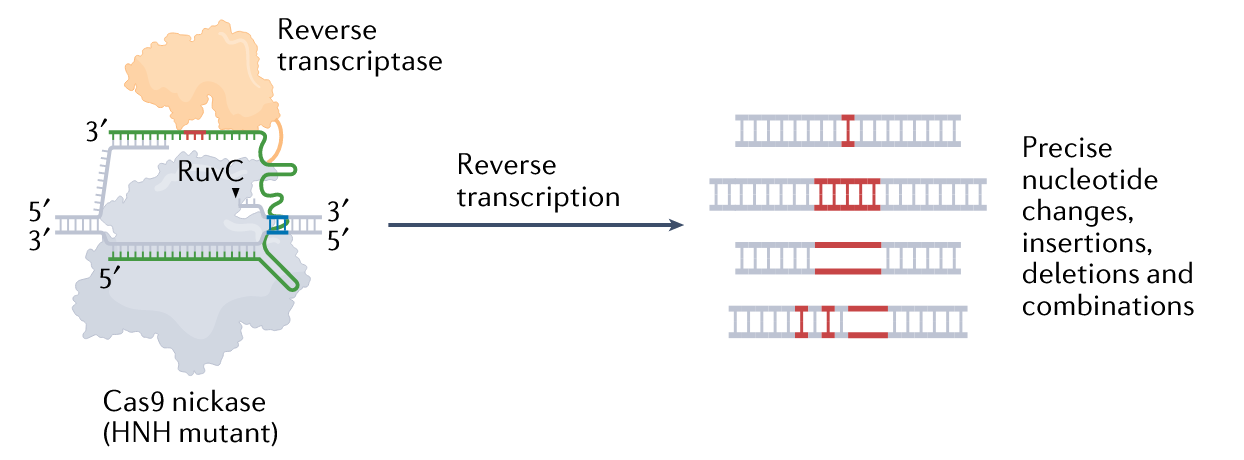
\includegraphics[width=\textwidth]{prime-editors-liu.png}
    \caption{Structure of prime editor, David R. Liu, et al 2019}
    \label{fig:prime-editors-liu}
\end{figure}

Prime editors are composed of a Cas9 nickase fused to a reverse transcriptase and a prime editing guide RNA(pegRNA), shown in \autoref{fig:prime-editors-liu}. The $5'$ end of the pegRNA contains a guide RNA(gRNA) that is complementary to the target DNA sequence(protospacer). The $3'$ end of the pegRNA contains a reverse transcriptase template that is complementary to the desired edit, as well as a Prime Binding Site(PBS) sequence used to hybridizing with the nicked strand. After the pegRNA binds to the target DNA, the Cas9 nickase nicks the non-binding strand of the DNA. The displaced nicked strand then hybridizes with the PBS at the $3'$ end of the pegRNA, allowing the reverse transcriptase to perform the edits. The reverse transcriptase uses the transcriptase template provided by the pegRNA to synthesize the desired edit into the nicked DNA strand. After the reverse transcription finishes, the nicked DNA strand is repaired by the cell's endogenous repair system, resulting in the desired edit successfully introduced to the genome\cite{liudavidr.SearchandreplaceGenomeEditing2019}. Some PE systems utilize an extra gRNA(sometimes called nick guide RNA, ngRNA) to increase the editing efficiency by also nicking the non-edited stand, prompting the cell's repair system to repair the unnicked strand using the edited strand as template\cite{liudavidr.SearchandreplaceGenomeEditing2019}. The process of prime editing is visualized in \autoref{fig:prime-editing}.

\begin{figure}[ht]
    \centering
    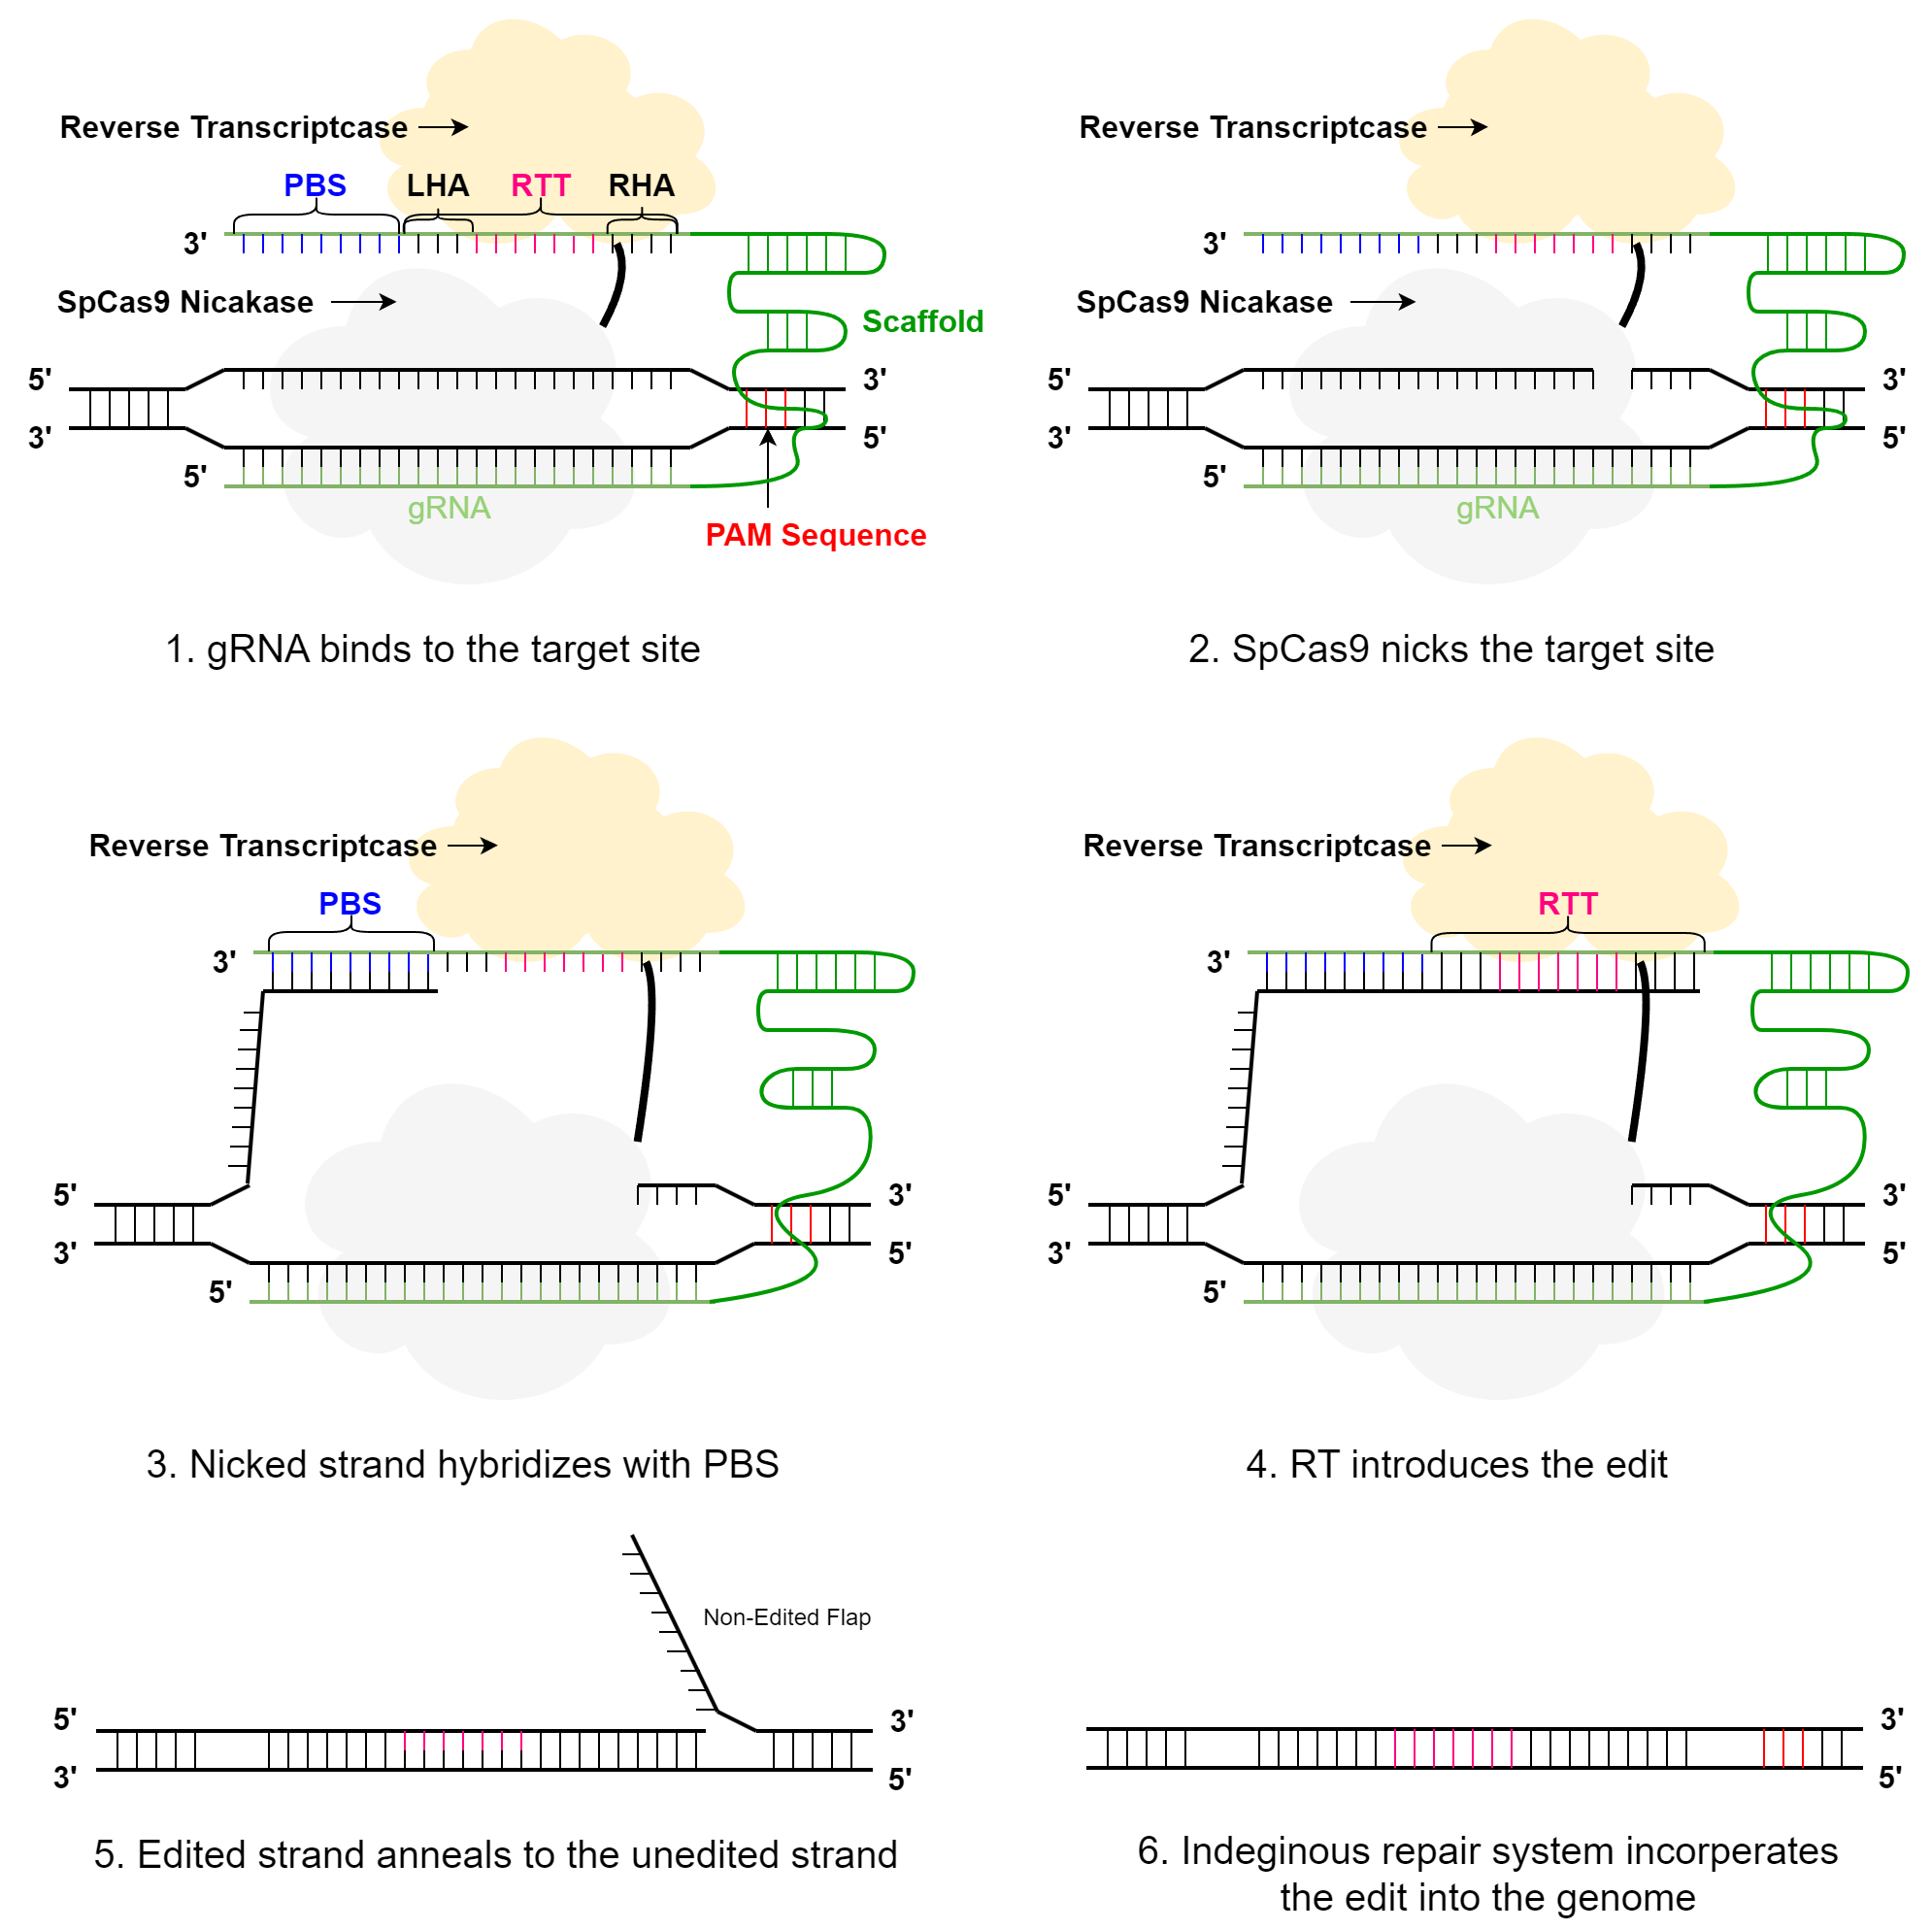
\includegraphics[width=\textwidth]{prime-editing-process.png}
    \caption{Prime Editing Process, David R. Liu, et al 2023}
    \label{fig:prime-editing}
\end{figure}

\section{General Open Questions and Selection of Particular Question for Study}

The design of pegRNA is of crucial importance to the success of prime editing. For the same target DNA sequence and desired edits, different pegRNAs can result in different editing efficiencies. Empirical methods that laboriously test a large number of pegRNAs to find the most efficient one  are time-consuming and expensive. As a result, it would be very beneficial to be able to perform in silico prediction of the efficiency of pegRNA given a target DNA sequence and desired edits. 

In silico guide design has proven to be effective for other precision editing tools including CRISPR-Cas9 HDR and base editors\cite{chenGenomewideCRISPROfftarget2023,marquartPredictingBaseEditing2021}. However, the design of pegRNA is significantly more complicated, as pegRNA contains the PBS sequence and reverse transcriptase template, in addition to the single guide RNA(sgRNA) used in other tools. PE3 also has a ngRNA that needs to be designed. At the same time, prime editing is a complex multiple step process where each step of the prime editing process can affect the result of the subsequent procedures. For example, if the PAM sequence is edited by the reverse transcriptase, the Cas9 nickase would not be able to rebind and nick the edited strand before the complementary strand is repaired. This would result in higher editing efficiency with less off-target effects. The model would need to be able to capture the interactions between the different components of the prime editing system and the target DNA sequence to make accurate predictions.

As a result, the exact determinants of prime editing efficiency are still not fully understood, and the question of predicting the efficiency of prime editing given a target DNA sequence and desired edits is still very much open. A number of designing tools used to propose candidate pegRNAs given target sequences by hardcoding design guide from the original PE paper have been developed, such as the PE-Designer\cite{hwangPEDesignerPEAnalyzerWebbased2021}. However, how to unbiasedly optimize the combination of all of these features from the design guide and identifying the most suitable sequence from a list of candidates remains problematic.

This problem inspired a population of machine learning methods, attempting to embed several known determinants of prime editing efficiency into the model architecture and produce superior results over the non-ML classical algorithms. Some examples are:

\begin{itemize}
    \item Easy-Prime, a gradient boosted tree model leveraging the result of DeepSpCas9 (convolutional neural network) for sgRNA efficiency prediction\cite{liEasyPrimeMachineLearning2021,kimSpCas9ActivityPrediction2019}
    \item PREDICT, an attention-based recurrent neural network model\cite{schwankgeraldPredictingPrimeEditing2023}
    \item DeepPrime, a convolutional neural network model, also taking the result of DeepSpCas9 as input\cite{kimPredictingEfficiencyPrime2021a}
\end{itemize}


This study aims to follow the steps of the aforementioned algorithms and tackle the problem of predicting the efficiency of prime editing given a target DNA sequence and desired edits, leveraging the ever growing dataset of prime editing outcomes produced by high-throughput sequencing as well as the advancements and discoveries made by the machine learning algorithms.

\section{Proposed Method}

Starting from the simplest possible improvement, I'll first investigate the effect of a new tokenizer on the existing machine learning algorithms. Chen et al proposed a machine learning algorithm for predicting genome wide off target efficiency prediction. In their study, they came up with an advanced tokenizer, ``CRISOT-FP". When compared to the traditional one-hot encoding of wild-type and edited sequences, this tokenizer managed to achieve much superior performance on a gradient boosted tree implementation\cite{chenGenomewideCRISPROfftarget2023}. I'll swap the tokenizer in the existing machine learning algorithm with CRISOT-FP and see if it also results in better prediction accuracy.

Some more sophisticated architecture proven to be useful in the task of predicting the efficiency of other precision editing tools can also be implemented here, an example of which is the transformer architecture. Transformers have been very effective in BE-DICT, a machine learning algorithm for predicting base editing efficiency with performance surpassing that of CNN and Multi-layer perceptron\cite{marquartPredictingBaseEditing2021}. I'll implement an advanced model and train it on the same dataset to see if it can achieve better performance than the existing machine learning algorithms.

Ensemble learning is also an interesting direction. After having trained and modified a number of existing machine learning algorithms, I'll combine them into an ensemble model. The ensemble model will take the predictions of the individual models as input and output the final prediction. This is expected to improve the prediction accuracy of the individual models.

\section{Draft Timetable}

The following is a draft timetable for the project:

\begin{tabularx}{\textwidth}{X|c}
    \hline
    \textbf{Task} & \textbf{Due Date} \\
    \hline
    Literature Review & May 1st \\
    \hline
    Implementing Attention-based RNN model \textbf{PREDICT} in G. Schwank, et al\cite{schwankgeraldPredictingPrimeEditing2023} & May 20th$\sim$ May 27th \\
    \hline
    Adapting \textbf{PREDICT} with CRISOT-FP tokenizer & June 1st \\
    \hline
    Adapting other machine learning algorithms if successful on \textbf{PREDICT}\cite{liEasyPrimeMachineLearning2021,kimPredictingEfficiencyPrime2021a} & June 15th \\
    \hline
    Implementing advanced ML model such as the transformers and train it for the task & July 1st$\sim$ July 15th \\
    \hline
    Implementing ensemble learning with the selected models implemented during the study & Aug 1st \\
    \hline
    Testing and evaluation & Aug 7th \\
    \hline
    Finishing report & Sep 1st \\
    \hline
\end{tabularx}

Note that as suggested in the handbook, the report writing is done in parallel with the project. The due date is simply the date when the report is expected to be finished and reviewed.

Similarly, the testing and evaluation are done after each model is trained so that I can verify my implementation and make necessary modifications. The final testing and evaluation listed in the timetable is a systematic evaluation of all the models produced during this study.

\section{Supervisor Sign-off}

\begin{tabular}{@{}p{1in}p{4in}@{}}

\\
\\
Approved: & \\
&\hrulefill \\
& Peter Minary, Ph.D. \\
\end{tabular}

\newpage

\printbibliography

\end{document}